%----------------------------------------------------------------------------------------
%
% LaTeX-template for degree projects at LNU, Department of Computer Science
% Last updated by Johan Hagelbäck, Mar 2017
% Linnaeus University
%
% License: Creative Commons BY
%
%----------------------------------------------------------------------------------------

%----------------------------------------------------------------------------------------
%	Settings and configuration
%----------------------------------------------------------------------------------------

\documentclass[a4paper,12pt]{article}

\usepackage[T1]{fontenc}
\usepackage{times}
\usepackage[english]{babel}
\usepackage[utf8]{inputenc}
\usepackage{dtklogos}
\usepackage{wallpaper}
\usepackage[absolute]{textpos}
\usepackage[top=2cm, bottom=2.5cm, left=3cm, right=3cm]{geometry}
\usepackage{appendix}
\usepackage[nottoc]{tocbibind}
\usepackage[colorlinks=true,
            linkcolor=black,
            urlcolor=blue,
            citecolor=black]{hyperref}

\setcounter{secnumdepth}{3}
\setcounter{tocdepth}{3}

\usepackage{sectsty}
\sectionfont{\fontsize{14}{15}\selectfont}
\subsectionfont{\fontsize{12}{15}\selectfont}
\subsubsectionfont{\fontsize{12}{15}\selectfont}
\usepackage{placeins}
\usepackage{csquotes} % Used to handle citations

\renewcommand{\thetable}{\arabic{section}.\arabic{table}}  
\renewcommand{\thefigure}{\arabic{section}.\arabic{figure}} 

%----------------------------------------------------------------------------------------
%	
%----------------------------------------------------------------------------------------
\newsavebox{\mybox}
\newlength{\mydepth}
\newlength{\myheight}

\newenvironment{sidebar}%
{\begin{lrbox}{\mybox}\begin{minipage}{\textwidth}}%
{\end{minipage}\end{lrbox}%
 \settodepth{\mydepth}{\usebox{\mybox}}%
 \settoheight{\myheight}{\usebox{\mybox}}%
 \addtolength{\myheight}{\mydepth}%
 \noindent\makebox[0pt]{\hspace{-20pt}\rule[-\mydepth]{1pt}{\myheight}}%
 \usebox{\mybox}}

%----------------------------------------------------------------------------------------
%	Title section
%----------------------------------------------------------------------------------------
\newcommand\BackgroundPic{
    \put(-2,-3){
    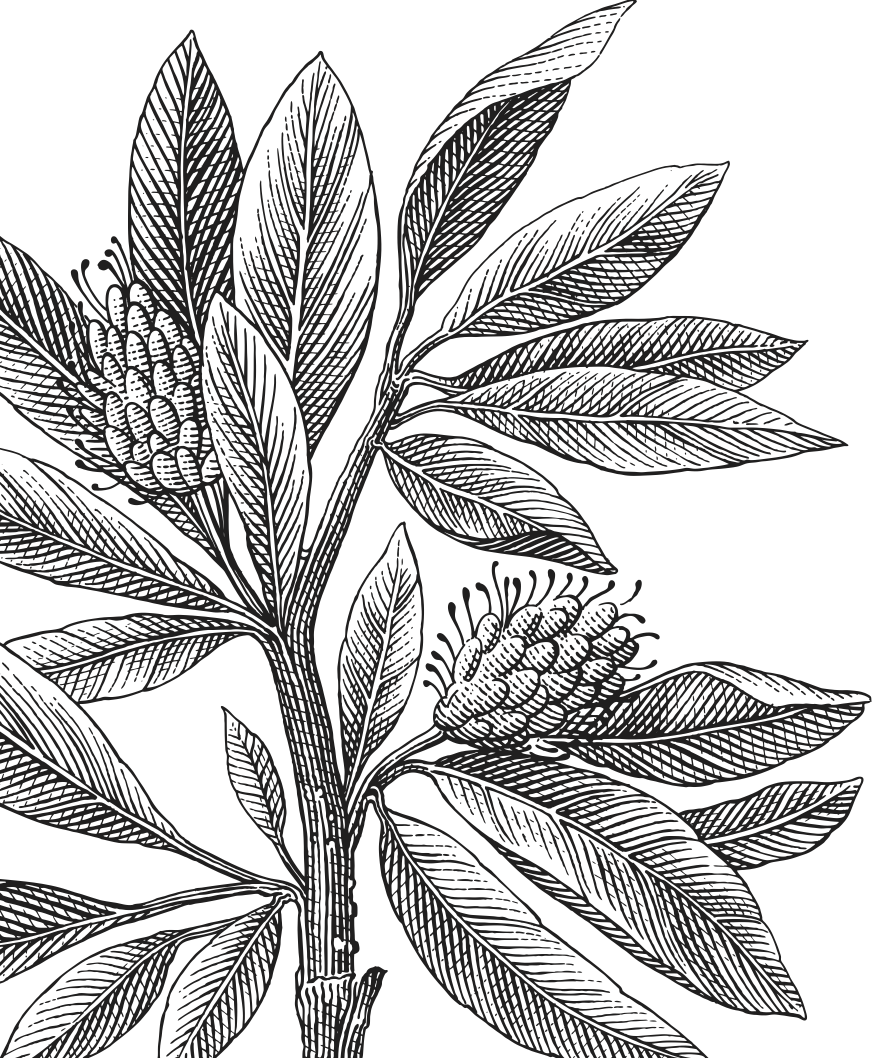
\includegraphics[keepaspectratio,scale=0.3]{img/lnu_etch.png} % Background picture
    }
}
\newcommand\BackgroundPicLogo{
    \put(30,740){
    
\includegraphics[keepaspectratio,scale=0.10]{img/logo.png} % Logo in upper left corner
    }
}

\title{	
\vspace{-8cm}
\begin{sidebar}
    \vspace{10cm}
    \normalfont \normalsize
    \Huge Bachelor Degree Project \\
    \vspace{-1.3cm}
\end{sidebar}
\vspace{3cm}
\begin{flushleft}
    \huge Evaluation of improvement measures of DNS Privacy\\ 
    \it \LARGE - Protection towards Web filters 
\end{flushleft}
\null
\vfill
\begin{textblock}{6}(10,13)
\begin{flushright}
\begin{minipage}{\textwidth}
\begin{flushleft} \large
\emph{Author:} Songho Lee\\ % Author
\emph{Supervisor:} Ola Flygt\\ % Supervisor
%\emph{Examiner:} Dr.~Mark \textsc{Brown}\\ % Examiner (course manager)
\emph{Semester:} VT 2019\\ % 
\emph{Subject:} Computer Science\\ % Subject area
\end{flushleft}
\end{minipage}
\end{flushright}
\end{textblock}
}

\date{} 

\begin{document}
\pagenumbering{gobble}
\newgeometry{left=5cm}
\AddToShipoutPicture*{\BackgroundPic}
\AddToShipoutPicture*{\BackgroundPicLogo}
\maketitle
\restoregeometry
\clearpage
%----------------------------------------------------------------------------------------
%	Abstract
%----------------------------------------------------------------------------------------
\selectlanguage{english}
\begin{abstract}
\noindent Current usage of the DNS system is the most significant loophole of Internet users' privacy, as all queries and answers for resolving web address are not protected in most cases. % Thesis statement, background description
Lack of confidentiality in the DNS system enables everyone who has control of the path between a user and DNS resolver can collect someone's usage pattern and fingerprint him and filter his access to specific websites. % Motivation
Despite a single solution for addressing privacy risks in all stages of the DNS query process does not exist, the report acquaints several Internet standardisations for DNS privacy that are complementary to the existing DNS system and verifies that implementation of these brings significant enhancement of users' privacy.
%The report explores existing methods to enhance DNS Privacy and sets up a series of experiments to verify implementations of such methods for privacy enhancement. % Description of problem explored
\\\\
\textbf{Keywords: DNS, DNS-over-https, DNS-over-TLS, Privacy}
\end{abstract}

%----------------------------------------------------------------------------------------
%	Preface
%----------------------------------------------------------------------------------------
%\newpage
%\textbf {\large{Preface}}\\

%\noindent You can have a preface in the report if you want, but it is not necessary. In this you can write more personal reflections on your degree project. In the preface you can also take the opportunity to thank the people who have been particularly helpful during the report writing, for example if you had any contact with a company that helped with the project, people that guided or helped you during the project, or your family and friends that supported you during the project. The preface shall not be longer than half a page.

%----------------------------------------------------------------------------------------
\newpage
\pagenumbering{gobble}
\tableofcontents % Table of contents
\newpage
\pagenumbering{arabic}

%----------------------------------------------------------------------------------------
%
%	Here follows the actual text contents of the report.
%
%----------------------------------------------------------------------------------------

\section{Introduction}
This chapter describes what Doname Name System (DNS) is, and how the legacy design of DNS has become a privacy threat. Before diving into the privacy risks of DNS, the background section introduces relevant structure and mechanisms. Knowledgable readers in DNS and Client subnet function may leap to section \ref{problemformulation}.

\subsection{Background}
Digital transformation has brought things used to be done in real life decades ago to the online. At work, people have a video conference call instead of a business trip if not necessary. For shopping goods, people fill in credit card numbers for cross-border payments rather than visiting a bank branch to issue paychecks. In other words, the stage where people work now has been shifted to cyberspace in recent decades, and the Internet has become an essential part of the people.

Despite the ubiquitousness of the Internet, users' activities online are collected under pervasive monitoring by different actors.
Pervasive Monitoring means ``widespread attack on privacy\cite{rfc7258}.'' Information collected in such action could lead to a breach of users’ privacy, by re-identifying users based on traffic\cite{herrmann2010analyzing}, or could become aids for launching an active form of attacks, such as masquerade and denial of service.
Unfortunately, insecure architecture of Domain Name System allows the pervasive monitoring, and thus it should be mitigated. Before discussing the privacy problems of DNS, we introduce DNS and its components which are important to adress.

\subsubsection{DNS}
Every activity on the web most likely begins with entering a human-friendly domain name in the web-browser. Once we enter a domain name for visiting a website, DNS resolves the address to an actual Internet Protocol Address of a web server which hosts the website. In case multiple websites are hosted on a single server, the entered fully qualified domain name(FQDN) is used to differentiate virtual hosts on a web server\cite{virtual24host}. Therefore, DNS is a critical component of the Internet.
%What about describing hjierarchical structure of Domain Name System here?
\subsubsection{DNS Servers}
DNS servers consist of four types: Stub resolver, Recursive resolver, Authoritative server, and Forwarding DNS server. Resolvers refer to programmes that obtain information from name servers upon clients' requests\cite{rfc1034}.

Stub resolver is a resolver that serves as an entry-point of querying DNS from applications and directs search request to the nearest recursive resolver\cite{rfc1123}. As it cannot complete domain name resolution by itself, stub resolver is dependant on a recursive resolver\cite{rfc8499}.

Recursive resolver is a server which receives a DNS query from a stub resolver and gets the final answer to the query, by (1) answering from its local cache or (2) sending queries to other DNS servers\cite{rfc8499}. After a recursive resolver has sent query request to other authoritative name servers, it is expected for the resolver to store the answer as a local cache. It is the first server in DNS query flow that contacts other servers to get the answer for the client. 

Authoritative (name) server is a server that has ``authority over one or more DNS zones\cite{rfc8499}'' and ``can answer queries without needing to query on other servers as it knows the content of the queried DNS zone by local knowledge\cite{rfc2182}.''

DNS forwarding server is a server that forwards queries to recursive resolver or other forwarding server. It does not perform query process for the stub resolver.
\subsubsection{DNS Query process}
Due to the hierarchical structure of the Domain Name System with delegations of authorities \cite{rfc1591}, getting the exact IP address of a given domain name involves several DNS servers. Figure \ref{queryprocess} shows an example of querying ``saimei.ftp.acc.umu.se.''. 
\begin{figure}[ht!]
    \begin{center}
        \includegraphics*[width=\columnwidth]{img/dnsquery}
    \end{center}
    \caption{DNS Query sequence diagram}
    \label{queryprocess}
\end{figure}
In the diagram, steps 2 and 3 returns top-level-domain(TLD) from the root servers. the steps 4 and 5 obtain the Authoritative name server of Swedish TLD. The .SE TLD returns name server of Ume\aa\ University in steps 6 and 7. In the last, the name server of umu returns IPv4 address (A record) of the given address, so that recursive resolver can provide the answer to the stub resolver. These steps are performed under the assumption that none of the queries is cached. 
\subsubsection{EDNS(0) and Client Subnet}
The extension mechanisms for DNS (EDNS) is specified in RFC 6891. EDNS allows both DNS servers and client to send ``larger DNS packet than the original 512 octet limit \cite{rfc6891}'', so that it benefits of utilising larger size. It makes sending long IPv6 address and possible DNSSEC signatures. As of February 2019, major DNS resolver operators have started not to support non-EDNS compliant servers. 

EDNS(0) provides several options, and one of the option is Client Subnet(ECS) feature, as described in RFC 7831 \cite{rfc7871}. When ECS is used, recursive DNS servers provide a truncated client IP address in its DNS queries to the upstream authorities to permit "topologically localised answers for Content Delivery Networks (CDN)\cite{kintis2016understanding}".

\subsection{Related work}
The project accredits pioneer research of "DNS Privacy Considerations (RFC 7626) \cite{rfc7626}" which has provided theoretical foundations in analysis of DNS privacy. 
As of 2019, there are number of studies are presented to mitigate privacy issues based on the analysis. These studies are later presented in Chapter 3.

Survey of DNS privacy enhancing methods are presented by P. Werneck and J.H.C. van Heugten. P. Werneck evaluated approaches to improve privacy of DNS and stated limitations of identified approaches\cite{werneck2014dns} in 2014. J. Heugten evaluated exisiting solutions to ehnance DNS Privacy in 2018 in his study \cite{van2018privacy}. As standariseation of DNS-over-HTTPS is recently finalised\cite{rfc8484}, study from van Heugten reflects more recent changes.

\subsection{Problem formulation}\label{problemformulation}
Currently, almost all DNS traffic is sent in clear text \cite{rfc7626} over the UDP protocol \cite{tcp2014analysis}, and it makes DNS queries vulnerable to being hijacked or used to filter users' traffic.
All participants of the DNS query process, as illustrated in Figure \ref{queryprocess}, transmit messages intensively, and these are in plaintext.
It is also noteworthy that all participating authoritative name servers receive the same questions, although it is not necessary for Authoritative servers in higher hierarchies in the process to know all the complete domain address in question.

S. Bortzmeyer has analysed that particular fields in DNS packet\cite{rfc1035} such as Query name (QNAME) and Source IP address reveal ``communication relationships\cite{rfc7626}''.
These series of observations indicate that there are risks of information leakage in following places: (1) tapping on the wire ``between the stub resolvers and the recursive resolvers'', and (2) information leaks in the servers.
The following research questions are formulated having regards to the privacy breaching circumstances.

\begin{table}[h!]
    \begin{tabular} {|p{1.2cm}|p{12.8cm}|} \hline
        \textbf{RQ1} & What methods exist to enhance DNS Privacy? \\ \hline
        \textbf{RQ2} & How does DNS Privacy improvement benefit users from being blocked by web filters?\\ \hline
        \textbf{RQ3} & What would be possible disadvantages or overheads with DNS Privacy enrichment? \\ \hline
    \end{tabular}
    \caption{Research questions}
\label{researchquestions}
\end{table}

\subsection{Motivation}
Most of the internet activities begin with DNS query, hence DNS is vital. Notwithstanding the importance of DNS, designers of the current DNS protocol have not taken consideration of ``confidentiality of protocol metadata''. Therefore DNS queries reveal communication flows, and this property of DNS protocol is used in different contexts by different actors. Examples of usages are traffic monitoring for network management or limiting the influence of malicious websites by DNS Footprinting of malware\cite{stoner2010dns}, or detecting malware infections\cite{lemos2013got}.

Other exemplary usages of this property of DNS are nation-state surveillance, privacy-unfriendly activities of commercial sectors\cite{weaver2011redirecting}, and illegal actions by criminals. Surveillance affects individuals to possess stress and anxiety\cite{oulasvirta2012long}, and behavioural changes like self-censorship \cite{rfc6973}. RFC 6973 connotes that Privacy harms involve ``harms to financial standing, reputation, solitude, autonomy, and safety\cite{rfc6973}'' of individuals.

S. Farrell et al. state in RFC 7258 that allowing monitoring by benevolent actors and defending privacy against nefarious actors do not hold hand in hand, as the actions required to achieve both, regardless of the motivations, are indistinguishable\cite{rfc7258}.
Disadvantages incurred by lack of DNS privacy significantly overweight advantages, and therefore DNS privacy should be mitigated in any feasible practices.

\subsection{Objectives}
The following objectives are set to answer the research questions and transform the tasks into the smaller pieces. Hereafter we denote Objective as O and research questions as RQ, and Table \ref{objectives} shows the objectives which we will discuss.
\begin{table}[h!]
    \begin{tabular} {|p{1.2cm}|p{12.8cm}|} \hline
        \textbf{O1} & Explore the state of arts in mitigative methods to enhance DNS Privacy \\ \hline
        \textbf{O2} & Verify application of DNS privacy-enhancing methods complicates DNS eavesdropping\\ \hline
        \textbf{O3} & Identify areas which the selected methods could not address. \\ \hline
        \textbf{O4} & Estimate factors that may lead to a load increase on recursive DNS resolvers by improving DNS Privacy.\\ \hline
    \end{tabular}
    \caption{Objectives}
    \label{objectives}
\end{table}

RQ1 derives O1; mitigative methods need to be studied to see which methods exist.
O2 and O3 are set to answer RQ2; to see whether the methods we find by performing O1 helps to secure the privacy or not will prove any possible benefits of the Internet users. O4 aims to answer RQ3.
\subsection{Scope/Limitation}
The project has a focus on improving privacy part, from the security perspectives. In other words, reflected to a Confidentiality, Integrity, Availability(CIA) triad, enhancing Integrity and availability perspective is not priortised in the current project. Issues and challenges of DNS security as whole may be found in other studies, such as one conducted by Ning Hu et. al.\cite{ning2017dnssecurity}. 

%You cannot solve everything. Here you describe what you do, and what you don't do, in your project. Limitations can for example be that you only compare some frameworks of all frameworks available on the market, that you only suggest an architecture for a specific software product and not a general architecture, or that you only include university students in a study and not a broader population sample.

\subsection{Target group}
The project aims to provide insight on DNS Privacy for Internet users and recursive resolver providers for improving users' privacy.
%Here you outline which target group that might be interested in your work. If you, for example, do a project about software architectures, a target group can be professional developers and architects that work with similar software systems as the system you investigated.

\subsection{Outline}
The report follows in Introduction, Methods, Results, and Discussion(IMRaD) pattern. However, as several scientific methods are chosen, which is described in the next chapter, the result and analysis parts are extended for each chosen scientific method. 

\newpage
\section{Method}
\label{Method}
This chapter describes the chosen scientific methods to answer the research questions (see Table \ref{researchquestions}) and meet the objectives (see Table \ref{objectives}).
The study was conducted by systematic literature review and controlled experiment, and the following sections motivate the choice of a scientific method for meeting objectives. 
\subsection{Literature review}
A systematic literature review was performed to accomplish \textbf{O1} and \textbf{O3}; to study mitigative methods of DNS privacy and identify areas of limitations.
Exploring the existing design suggestions or implementation for improving the confidentiality of DNS transactions needed to be done systematically, to eradicate biases and to minimise opportunities for not obtaining suitable solutions.

A search criterium was set to list articles that cited RFC 7626 from a database Google Scholar, as the analysis had provided a clear insight of DNS privacy issues\cite{rfc7626}, and since around four years had passed after its publication, it was anticipated that fellow researchers have tried to solve or list risks identified in the article.
%If the results based on the criteria is insufficient, inclusive criteria will be applied using search term such as DNS Privacy and DNS Security will be used. Exclusive criteria must be applied as well to limit the contents of the articles to be relevant to the defined problem. Therefore, any solving other security aspects of DNS, such as availability or integrity will be excluded.
\subsection{Controlled Experiment and Verification}
\textbf{O2} was accomplished by selecting securing methods that are near or already in practice and reproduce these in a controlled environment.
Due to this reason, it may have excluded some of the areas from \textbf{O1}. Verification, as defined in \textbf{O2}, was done by Examining DNS query and response packets between stub resolver and recursive resolver, after having applied privacy enhancive methods under the controlled environment.

\textbf{O3} was achieved by studying surveys from \textbf{O1} and empirical results from \textbf{O2}. \textbf{O4} was evaluated based on outcome of \textbf{O1} and \textbf{O2}.

\subsection{Reliability and Validity}
The study is seen to have reliability on the results of the literature review, as the same effect will be derived by performing a search as described in the previous section. As Appendix A includes the source code of the experiment scripts, a similar result is expected to be derived by other researchers as well. 

The project deployed its experiments in a virtualised environment to minimise unforeseen factors that would impact performance measurements.

\subsection{Ethical considerations}
The project performed experiments in a controlled environment to eliminate other affecting factors. It means that no real data of legal representatives are collected without his/her consent. 

\newpage
\section{Survey of DNS Privacy enhancing methods}
This chapter presents the result of a systematic literature review on studies related to DNS Privacy.
%Afterwards, the analysis of the result follows.
As the raw data from the Google scholar had contained several duplicated entries, duplicated studies were excluded. Series or revisions of the same article are marked as duplicated. For such cases, the proceeding study was chosen to present.
The analysis section which follows after this chapter motivates strategies for categorisation of raw search results.

\subsection{Improvement suggestions}
Studies shown in Table \ref{channel} attempted to secure the communication channel of the DNS query. In other words, these studies suggested applying Encipherment mechanism to deliver Connection Confidentiality as X.800 defines \cite{x800}.

\begin{table}[h!]
    \begin{tabular}{ | l | p{10.5cm} | l | l | }
        \hline
            ID & Title & Year & Cites  \\ \hline
            \cite{hu2016specification} & Specification for dns over transport layer security (tls) & 2016 & 27 \\ \hline
            \cite{rfc8484} & Dns queries over https (doh) & 2018 & 5\\ \hline
            \cite{reddy2017dns} & Dns over datagram transport layer security (dtls) & 2017 & 3\\ \hline
            \cite{bucuti2015opportunistic} & An opportunistic encryption extension for the DNS protocol & 2015 & 2 \\ \hline
            \cite{dickinson2018usage} & Usage profiles for dns over tls and dns over dtls & 2018 & 1 \\ \hline
            \cite{saraj2017design} & Design and implementation of a lightweight privacy extension of DNSSEC protocol & 2017 & 0 \\ \hline
            \cite{dnsoquic} & Specification of DNS over Dedicated QUIC Connections & 2019 & 0 \\ \hline
            \cite{denis2015dnscrypt} & DNSCrypt & 2015 & 0 \\ \hline
            \cite{dempsky2010dnscurve} & DNSCurve & 2009 & 0 \\ \hline
        \end{tabular}
        \caption{Literatures categorised as securing communication channel}
\label{channel}
\end{table}

Table \ref{content} summarised studies on minimising privacy breaching information in the content of packets generated in the DNS query process.
%The approach can be seen as metaphors of Least common mechanism and Isolation as described in security design principles. 

\begin{table}[h!]
    \begin{tabular}{ | l | p{10.5cm} | l | l |}
        \hline
            ID & Title & Year & Cites \\ \hline
            \cite{bortzmeyer2016dns} & DNS query name minimisation to improve privacy & 2016 & 33 \\ \hline
            \cite{annee-dprive-oblivious-dns-00} & Oblivious DNS - Strong Privacy for DNS Queries & 2019 & 0 \\ \hline
            \cite{pan2018mitigating} & Mitigating Client Subnet Leakage in DNS Queries & 2018 & 0 \\ \hline
        \end{tabular}
        \caption{Literatures categorised as securing content}
\label{content}
\end{table}

There are several pieces of research and design proposals of new architecture which would replace the current DNS system. These are found in Table \ref{architectures}

\begin{table}[h!]
    \begin{tabular}{ | l | p{10.5cm} | l | l | }
        \hline
            ID & Title & Year & Cites \\ \hline
            \cite{ambrosin2018security} & Security and privacy analysis of national science foundation future internet architectures & 2018 & 3 \\ \hline
            \cite{grothoff2017gnunet} & The GNUnet System & 2017 & 1 \\ \hline
            \cite{asoni2017paged} & A Paged Domain Name System for Query Privacy & 2017 & 0 \\ \hline
            \cite{loibl2014namecoin} & Namecoin & 2014 & 12 \\ \hline
        \end{tabular}
        \caption{Literatures categorised as Architectural proposal}
    \label{architectures}
\end{table}
\FloatBarrier
\subsection{Case studies on attack scenarios}
Several studies demonstrated privacy risks of the current DNS standard and proposed mitigative methods which we had introduced in the previous section. 

\begin{table}[h!]
    \begin{tabular}{ | l | p{10.5cm} | l | l | }
        \hline
            ID & Title & Year & Cites \\ \hline
            \cite{kirchler2016tracked} & Tracked without a trace: linking sessions of users by unsupervised learning of patterns in their DNS traffic & 2016 & 10 \\ \hline
            \cite{mohaisen2017leakage} & Leakage of. onion at the DNS Root: Measurements, Causes, and Countermeasures & 2017 & 3 \\ \hline
            \cite{grothoff2017nsa} & NSA's MORECOWBELL: knell for DNS & 2017 & 3 \\ \hline
            \cite{spaulding2018d} & D-FENS: DNS filtering \& extraction network system for malicious domain names & 2018 & 1 \\ \hline
        \end{tabular}
        \caption{Literatures categorised as demonstrating attack scenarios by exploiting the lack of DNS privacy}
\label{attacks}
\end{table}
%\subsection{Evaluation of the improvement suggestions by other researchers}

\section{Analysis of the survey result}
This section provides an analysis of the survey results.
The refined search results were categorised into the following fields: studies that suggested improving the security breach and investigations that demonstrated the security vulnerabilities.
We have further classified the privacy improving studies into ones securing the content and others enhancing the channel, based on the privacy risk analysis of RFC 7626.
S. Bortzmeyer, who is the author of RFC 7626 identified risk area of DNS privacy as the followings\cite{rfc7626}: 
\begin{enumerate}
    \item Data in the DNS request
    \item On the wire
    \item In the servers
    \item Re-identification and other Interferences
\end{enumerate}

\subsection{Securing the communication channel}
Communication channel encirpher methods, as we presented in Table \ref{content}, attempt to alleviate risks (2) on the wire. It also partially addresses risks of (4) re-identification depends on who the subject of the attacker is. 
However, we did not find the one simple solution for securing all communication paths of all involved parties of the DNS resolving. Therefore, it is noteworthy to consider the location of the DNS resolver and limitations of each suggested methods.

\subsubsection{Location of Recursive DNS resolvers}
Recursive DNS Resolvers can be on a local machine, one provided by the Internet Service Providers (ISP) and Public DNS servers. 

\subsection{Securing content}
The term we used ``securing content'' includes reduction of the risks (1) Data in the DNS request and (3) In the servers. 

\section{Design of controlled experiment}
It is common that you will develop something in your project. It can be a mobile app, a stand-alone application, a website, a game, etc. In this chapter you describe the software you have implemented. 

In some projects you don't develop anything, for example if you do a systematic literature review. In this case you remove this chapter.

\newpage

\section{Results}
In this chapter you show and describe your results. You shall only show the raw results without any analysis, and you shall not put any conclusions or opinions in the description of the results. Try to be as objective as possible. An example of results from an experiment comparing five sorting algorithms is shown in Table \ref{results} below.\\



\begin{center}
\begin{table}[ht]
\begin{center}
\begin{tabular}{ccccccc}
\hline
Run & Bubble & Quick & Selection & Insertion & Merge \\
\hline
1 & 17384 & 24 & 3258 & 3 & 30 \\
2 & 17559 & 21 & 3386 & 3 & 27 \\
3 & 17795 & 19 & 3344 & 4 & 28 \\
4 & 17484 & 20 & 3417 & 3 & 28 \\
5 & 17642 & 19 & 3358 & 3 & 30 \\
\hline
Average & 17572.8 & 20.6 & 3352.6 & 3.2 & 28.6 \\
\hline
%
\end{tabular}
\end{center}
\caption{Execution times for the five sorting algorithms on 100 000 random numbers between 0 and 10 000.}
\label{results}
\end{table}
\end{center}

What you show heavily depends on the type of method you use and what type of data you collect. Numerical data can for example be shown in both tables and graphs. A complementary graph for the sorting algorithms example is shown in Figure \ref{graph}. For a questionnaire you can show the frequency (how many participants that selected the same answer) of each possible answer to a question.

\begin{figure}[ht!]
\begin{center}
\includegraphics*[width=0.6\columnwidth]{img/graph}
\end{center}
\caption{Execution times for the five sorting algorithms shown as a graph.}
\label{graph}
\end{figure}

Note that Tables and Figures shall be labeled with chapter.number, for example Table 4.1 and Figure 1.6.

\newpage
	
\section{Analysis}
Here you give meaning to and your own opinions of the results. What conclusions can you draw from the results? It is important that you don't draw any conclusions that cannot be backed up by your data. Consider using statistical tests to back up your claims. You can read about statistical testing \href{https://coursepress.lnu.se/subject/thesis-projects/statistical-testing/}{here}. 
	
\newpage
	
\section{Discussion}
The project intensively examines securing Domain Name queries as a method of enhancing end-users' privacy towards pervasive monitoring.
\subsection{Is securing DNS enough to protect users' privacy?}
A Question may arise why it mainly focuses on securing DNS although there exist other factors which disclose users' privacy.
To answer the question, let us have an example of a web filter, as it is a commonly found practical example of the large scale monitoring\cite{murdoch2008tools}.
%As web filters require monitoring of users' traffic to enforce its policy of restrictions, understanding the mechanisms of the web filter suits this context.

Web filter, also known as content-control software, is software that restricts access to a content that is delivered on the Web.
Wazen et. al categorise mechanisms of legacy web-filtering into five techniques: (a) Port-based, (b) DNS, (c) IP Address, (d) Certificate, (e) Payload-based (f) HTTP proxy filtering techniques\cite{shbair2015efficiently}.
Except for the technique based on DNS filtering, the rest methods are regarded as well-mitigated due to recent developments of the web environment. 

Among the various types of filtering techniques mentioned above, methods (a) and (c) are considered less efficient due to changes in the Internet ecosystem in recent decennial;
Internet firms such as Google, Facebook and Amazon show strong presence\cite{haucap2014google}, and the phenomenon may have reduced the diversity of traffic endpoint's IP addresses.
Moreover, it has become more common to have web services deployed in cloud environments\cite{clouds2018stat}, and IaaS providers extensively use ``Virtual Host\cite{virtual24host}'', which means various Web servers correspond to the same IP address.
It also eliminates the need for utilising different ports to co-host services. Thus, port usages are normalised.

Also, another notable change of the Internet is that adoption of HTTPS on the web has increased significantly\cite{felt2017measuring}.
The change has increased costs of performing technique (e) and brought challenges in payload-based traffic classification \cite{xue2013traffic}.
Also, it has made (f) less applicable, as a proxy does not directly process encrypted traffics\cite{shbair2015efficiently}.
Furthermore, the combination of wide deployment of HTTPS and Virtual Hosting has made technique (e) inefficient, because ``many companies share the same certificate across different services and domain names\cite{shbair2015efficiently}''.

However, the trend change of Internet has not brought additional challenges to Domain Name System (DNS) filtering. Therefore, the project studies to remedy the weakest point towards users' privacy, which in this case is DNS.

\subsection{Ethical dilemma of privacy enhancement; Liberation of illegal crimes?}
\newpage
		
\section{Conclusion}
In this chapter you end your report with a conclusion of your findings. What have you shown in your project? Are your results relevant for science, industry or society? How general are your results (i.e. can they be applied to other areas/problems as well)? Also discuss if anything in your project could have been done differently to possibly get better results. 

This chapter is also written in present tense.

\subsection{Future work}
You cannot do everything within the limited scope of a degree project. Here you discuss what you would do if you had continued working on your project. Are there any open questions that you discovered during the project work that you didn't have time to investigate?

\newpage


%----------------------------------------------------------------------------------------
%	References. IEEE style is used.
%
%----------------------------------------------------------------------------------------
\newpage

\hypersetup{urlcolor=black}
\bibliographystyle{IEEEtran}
\bibliography{references}
\newpage
%----------------------------------------------------------------------------------------
%	Appendix
%-----------------------------------------------------------------------------------------
\pagenumbering{Alph}
\setcounter{page}{1} % Reset page numbering for Appendix
\appendix

\section{Appendix 1} 
In the appendix you can put details that does not fit into the main report. Examples are source code, long tables with raw data and questionnaires.

\end{document}
